\artikel{Mensa - the cafeteria}
{The cafeteria at TU Darmstadt is referred to as "Mensa" in German.
Here you can get food from 11.15 to 14.00 .
}{


\noindent\textbf{Symbol explanation}
Each meal is signed with symbols to show you what they contain.

\begin{tabular}{|c|c|p{3cm}|}
\hline
\rule{0pt}{1cm+1ex}
\includegraphics[scale=0.5]{../grafik/artikel/vegetarian} & (V) & Vegetarian meal. It doesen't contain meat but can contain milk products or eggs.\\
 \hline
\rule{0pt}{1cm+1ex}
\includegraphics[scale=0.5]{../grafik/artikel/vegan} & (Vegan) & Vegan meals don't contain any animal products.\\
 \hline
\rule{0pt}{1cm+1ex}
\includegraphics[scale=0.5]{../grafik/artikel/chicken} & (G) & These meals contain chicken.\\
 \hline
\rule{0pt}{1cm+1ex}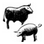
\includegraphics[scale=0.5]{../grafik/artikel/porkandbeef} & (S, R) & Theses meals contain pork or beef.\\
 \hline
\rule{0pt}{1cm+1ex}
\includegraphics[scale=0.5]{../grafik/artikel/fish} & (F) & These meals contain fish.\\
 \hline
\end{tabular}


}{Johannes Alef}